\begin{frame}
	\frametitle{Load and fixture specification}
	\begin{minipage}{0.85\textwidth}
		\begin{itemize}
		\item Boundary conditions requided - how to specify?
		\end{itemize}
	\end{minipage}
	\begin{minipage}{0.14\textwidth}
		\begin{figure}
			\scalebox{0.08}{
\includegraphics{Pictures/1CAD.pdf}}\\
			\scalebox{0.08}{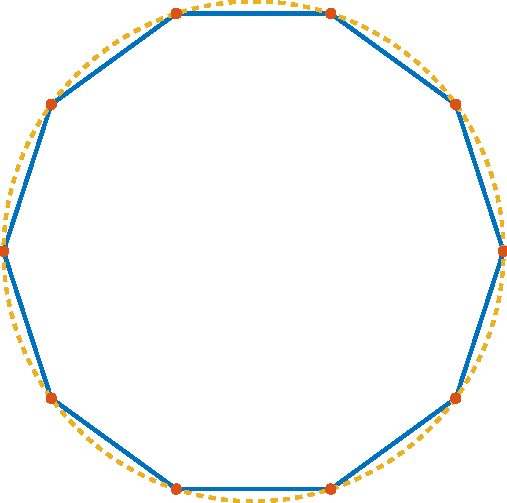
\includegraphics{Pictures/2STL.pdf}}\\
			\scalebox{0.08}{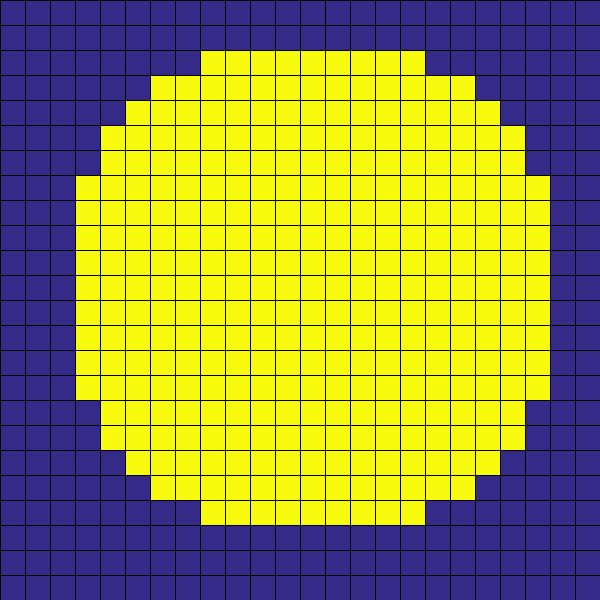
\includegraphics{Pictures/3VOX.pdf}}\\
			\scalebox{0.08}{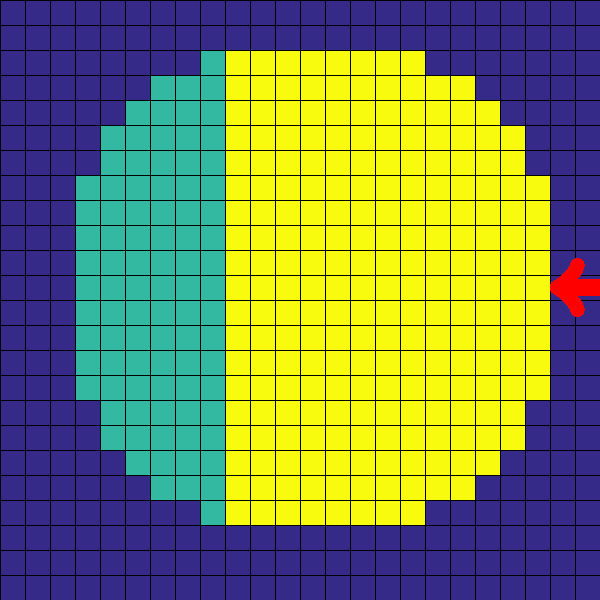
\includegraphics{Pictures/4TPD.pdf}}\\
			\scalebox{0.08}{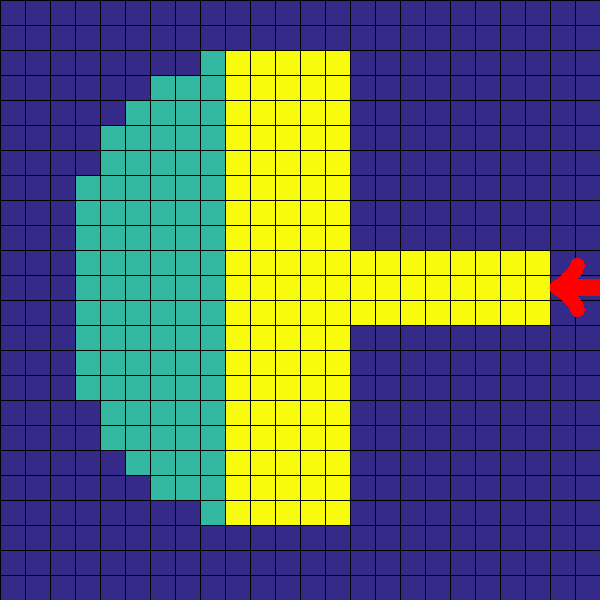
\includegraphics{Pictures/5TOPOPT.pdf}}\\
			\scalebox{0.08}{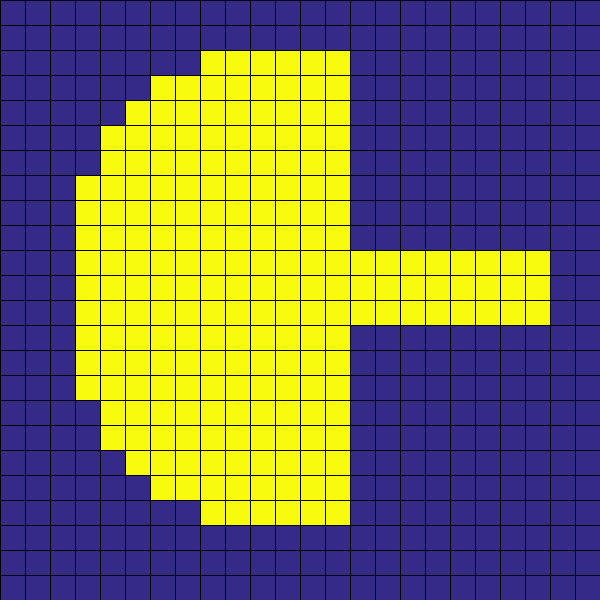
\includegraphics{Pictures/6TOPYOUT.pdf}}\\
			\scalebox{0.08}{
\includegraphics{Pictures/7MC.pdf}}
		\end{figure}
	\end{minipage}
\end{frame}
